\section{\textit{Octave Filter Bank}}

\textit{Octave Filter Bank} es un módulo compuesto por 8 filtros paso de banda cuyas frecuencias centrales están a distancia de octava, dentro del rango  $\SI{62.5}{\hertz}--\SI{8}{\kilo\hertz}$ (Estas frecuencias son algo más bajas que la nota do del sistema temperado). Según las especificaciones de EMS, estos filtros son resonantes. Aunque no trae más aclaraciones, podemos suponer que es precisamente el valor de dicha resonancia la que puede ser variada con cada dial. La función de este banco de filtros sería, por tanto, no la de hacer una ecualización multibanda, sino, más bien, la de colorear de una forma pronunciada el sonido de su input.

Esta configuración, sin embargo, no está libre de cuestiones difíciles de explicar: Llama la atención, por ejemplo, que estas frecuencias resonantes sean fijas en lugar de poder ser variadas por voltaje. Tampoco es claro qué anchura tiene la banda de cada filtro y cuál es su amplitud independientemente del valor de la de la frecuencia resonante. Por otra parte, el panel del Synthi 100 trae la siguiente descripción en el centro superior del módulo: \textit{Band Pass Centre Frequency (Hz)} (Fig. \ref{fig:octave_filter_bank}), lo cual no da ningún indicio de que se trate de un conjunto de filtros resonantes. Sin duda, estas cuestiones solo pueden dirimirse con la experimentación en el mismo sintetizador.

\begin{figure}
	\centering
	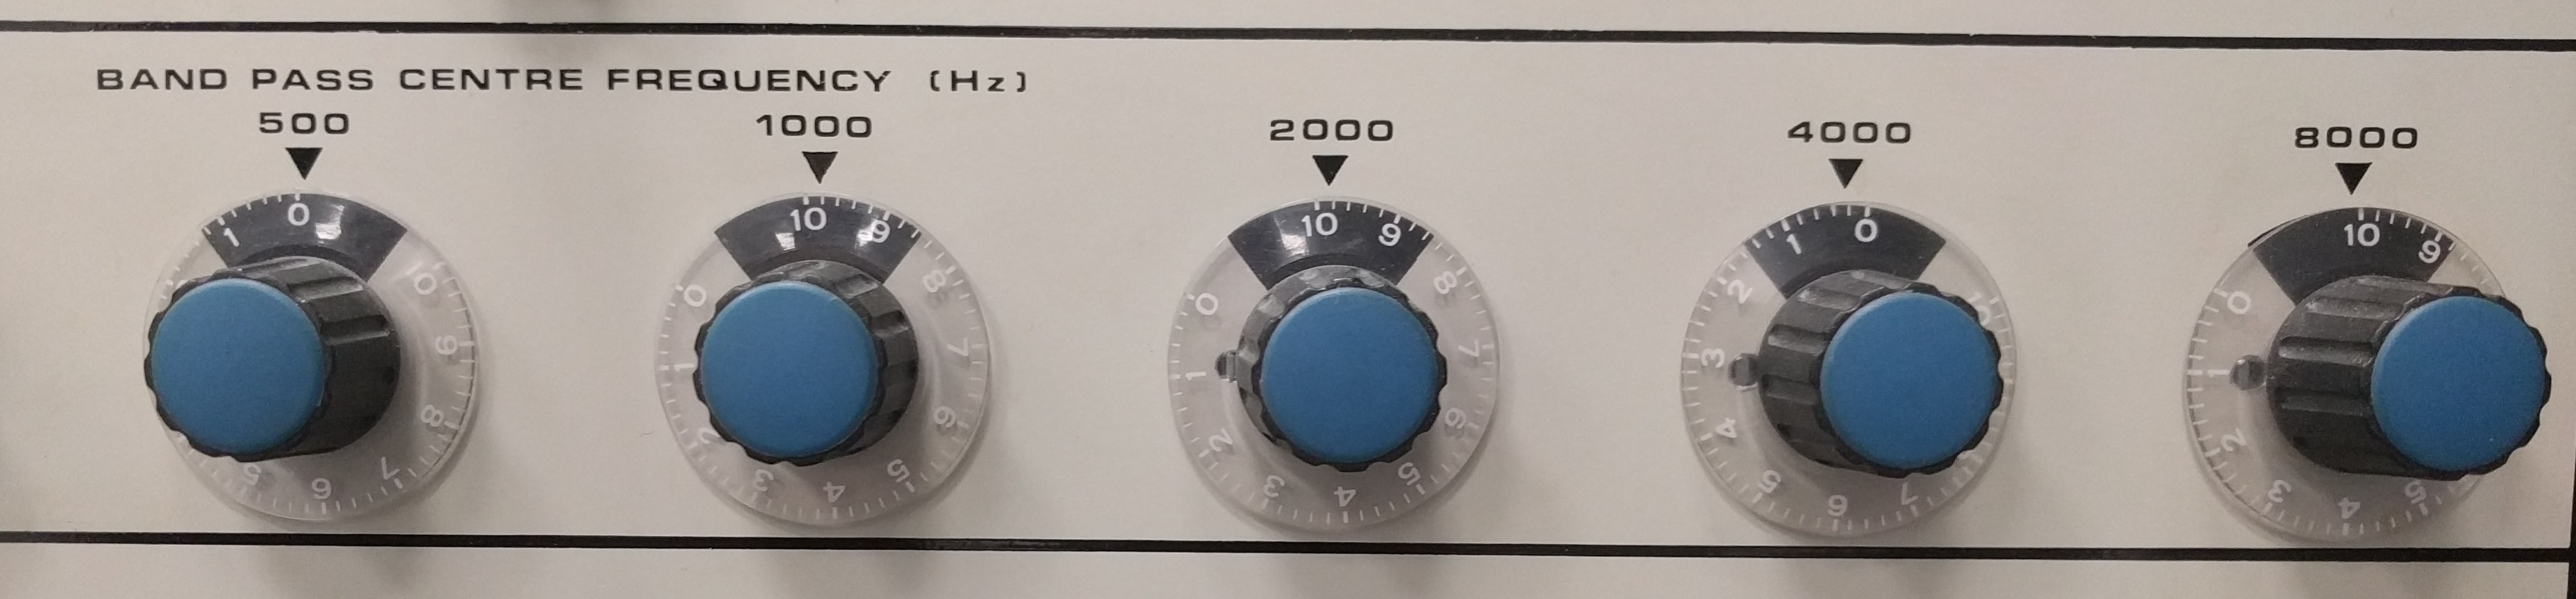
\includegraphics[width=1\textwidth]{images/octave_filter_bank}
	\caption[Módulo \textit{Octave Filter Bank}]{Vista parcial del módulo \textit{Octave Filter Bank}. Las frecuencias centrales de cada filtro están separadas entre sí por un intervalo de octava.}
	\label{fig:octave_filter_bank}
\end{figure}

\subsection{Implementación en \appName}

En el diseño del módulo en SuperCollider se ha optado por crear un filtro multibanda no resonante. Esta solución deja para estudios ulteriores el comportamiento real del módulo \textit{Octave Filter Bank} en el Synthi 100. Por otra parte, aunque no sea resonante, no cabe duda de que tiene la capacidad de sustraer de la señal del su input determinados rangos frecuenciales. En la versión presente de \appName, cada \textit{Synth} contiene como \textit{Ugen} principal a \texttt{BBandPass}, del conjunto de filtros \textit{BEQSuite}, un filtro paso de banda de segundo orden.

